\documentclass[conference]{IEEEtran}
\usepackage{cite}
\usepackage{amsmath,amssymb,amsfonts}
\usepackage{algorithmic}
\usepackage{graphicx}
\usepackage{textcomp}
\usepackage{xcolor}
\usepackage{hyperref}

\begin{document}

\title{OpenMP Parallelisation of a 3D Discrete Element Method Particle Simulator\\
\large Assignment 1}

\author{\IEEEauthorblockN{Bhukya Praveen Kumar}
\IEEEauthorblockA{\textit{Roll no : B23431}\\
Email: b23431@students.iitmandi.ac.in}
}

\maketitle

\begin{abstract}
This paper presents the development, verification, profiling, and parallelisation of a three-dimensional Discrete Element Method (DEM) solver for spherical particles. The solver computes translational motion using a linear spring-dashpot contact model and semi-implicit Euler time integration. OpenMP is utilized to parallelise the computationally dominant $O(N^2)$ particle-particle contact detection phase, yielding significant performance improvements. Verification against analytical solutions and performance scaling analysis are discussed.
\end{abstract}

\section{Introduction}
Discrete Element Method (DEM) simulations are computationally intensive due to the continuous tracking of particle trajectories and the resolution of inter-particle contacts. This work details a C++ implementation of a 3D DEM solver. We detail the physical and mathematical models, verify the serial implementation through standard test cases (free fall and particle bounce), and apply OpenMP directives to parallelise the solver for large particle systems ($N=5000$).

\section{Mathematical Formulation}
We consider $N$ spherical particles moving within a cuboidal domain. The translational motion of each particle $i$ is governed by Newton's second law:
\begin{equation}
m_{i}\frac{dv_{i}}{dt}=F_{i}, \quad \frac{dx_{i}}{dt}=v_{i}
\end{equation}
where $m_i$ is the mass, $v_i$ is the velocity, $x_i$ is the position, and $F_i$ is the total force. The total force comprises gravity, particle-particle contacts, and particle-wall contacts:
\begin{equation}
F_{i}=m_{i}g+\sum_{j\ne i}F_{ij}^{c}+F_{i}^{w}
\end{equation}

\section{Particle Contact Model}
The contact force $F_{ij}^c$ relies on a linear spring-dashpot model. For particles $i$ and $j$, the relative distance and normal vector are $d_{ij} = ||x_j - x_i||$ and $n_{ij} = (x_j - x_i)/d_{ij}$. Overlap is defined as:
\begin{equation}
\delta_{ij}=R_{i}+R_{j}-d_{ij}
\end{equation}
If $\delta_{ij} > 0$, a contact exists. With a normal stiffness $k_n$ and damping coefficient $\gamma_n$, the normal force to prevent nonphysical attraction is evaluated as:
\begin{equation}
F_{n}=\max(0,k_{n}\delta_{ij}-\gamma_{n}v_{n,ij})
\end{equation}
yielding the contact force vector $F_{ij}^{c}=F_{n}n_{ij}$.

\section{Numerical Algorithm}
The simulation advances using a semi-implicit Euler time integration scheme. At each timestep $\Delta t$, forces are evaluated based on current positions $x_i^n$ and velocities $v_i^n$, followed by state updates:
\begin{equation}
v_{i}^{n+1}=v_{i}^{n}+\frac{F_{i}^{n}}{m_{i}}\Delta t
\end{equation}
\begin{equation}
x_{i}^{n+1}=x_{i}^{n}+v_{i}^{n+1}\Delta t
\end{equation}

\section{Verification and Testing}
Before parallelisation, the serial solver was rigorously verified using standard baseline tests to ensure physical and mathematical accuracy.

\subsection{Free Fall}
A single particle dropped from rest follows the analytical trajectory $z(t)=z_{0}-\frac{1}{2}gt^{2}$. As shown in Fig. \ref{fig:freefall}, the numerical results generated by the C++ simulator align perfectly with the analytical solution.
\begin{figure}[htbp]
\centerline{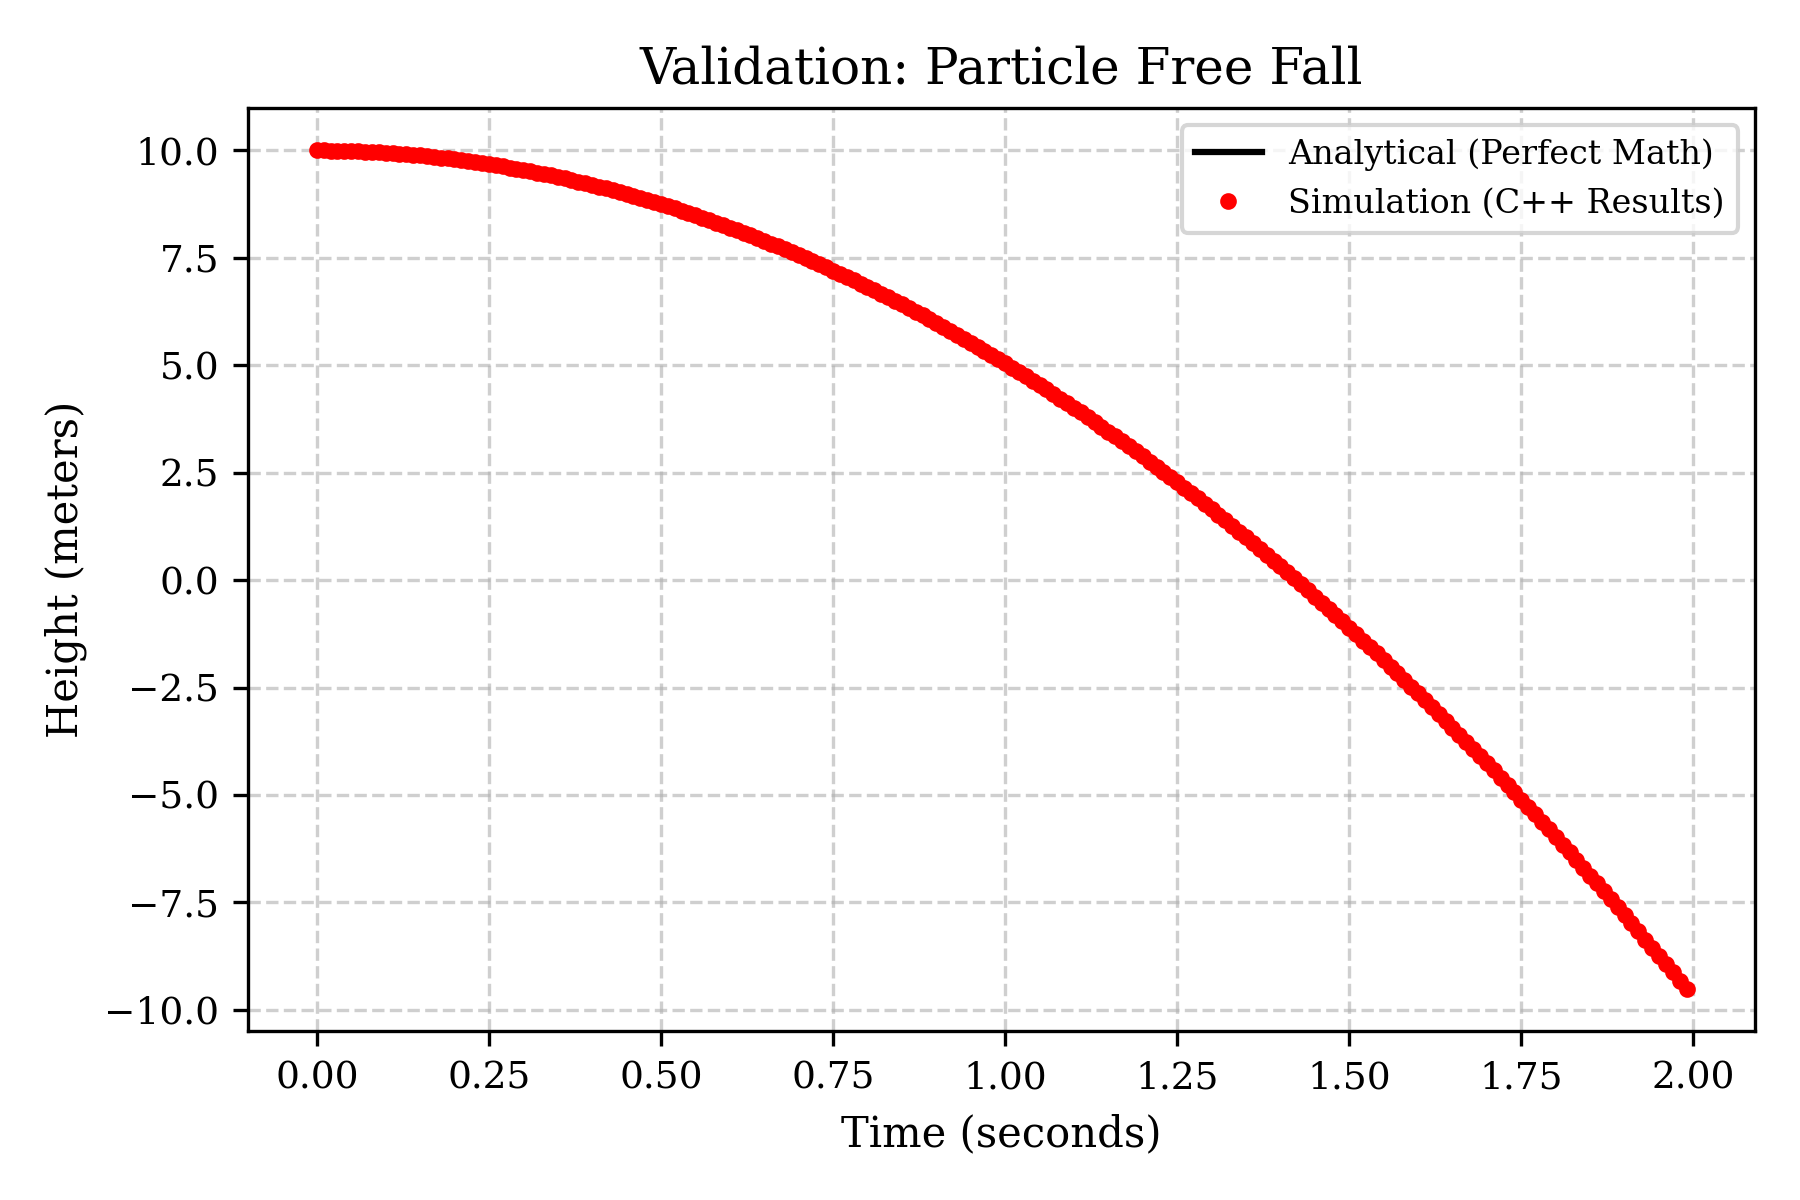
\includegraphics[width=\columnwidth]{my_freefall_plot.png}}
\caption{Numerical vs. Analytical solution for the free fall test.}
\label{fig:freefall}
\end{figure}

\subsection{Particle Bounce}
A particle dropped onto the lower wall rebounds using the specified spring-dashpot wall contact logic. The rebound height decays over time corresponding to the damping coefficient $\gamma_n$. Fig. \ref{fig:bounce} illustrates the energy dissipation, where kinetic energy peaks just before impact and decays as the particle slowly comes to rest.
\begin{figure}[htbp]
\centerline{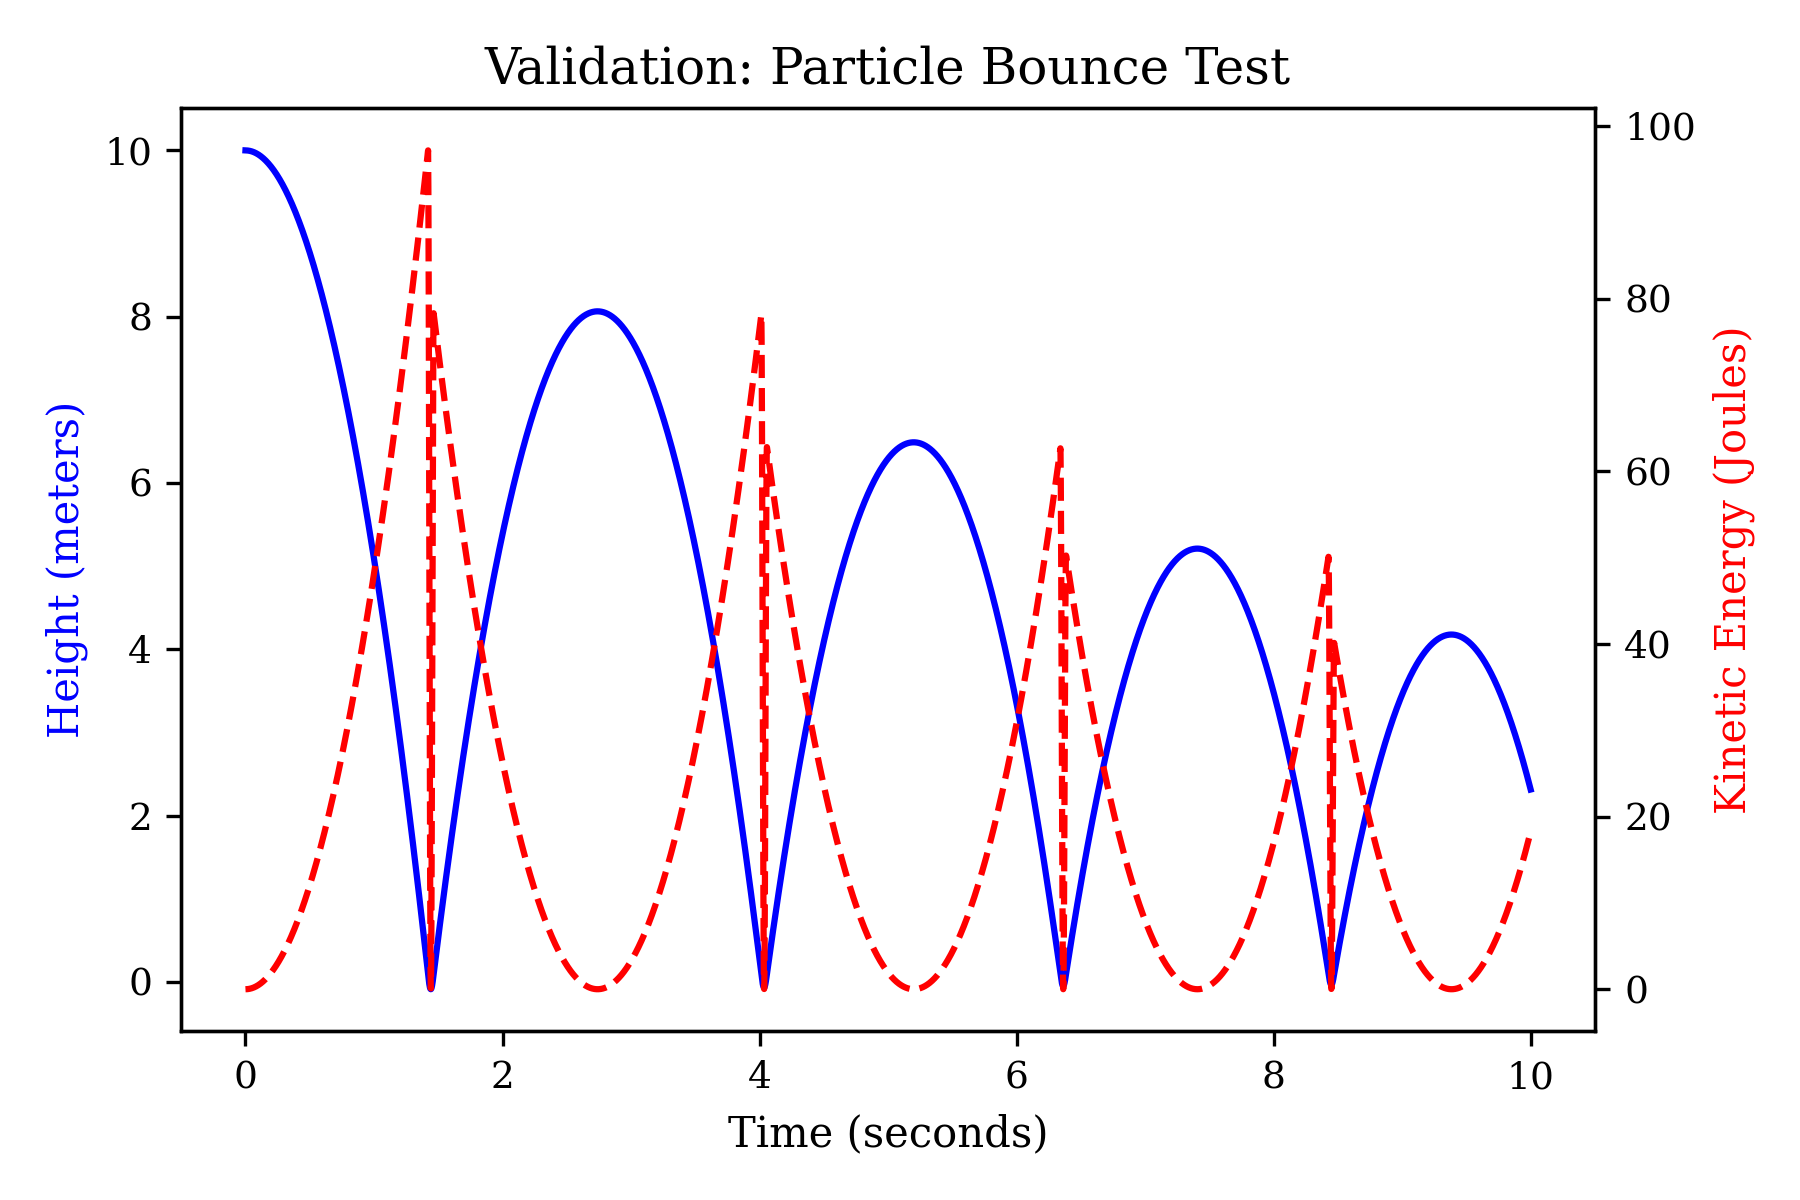
\includegraphics[width=\columnwidth]{my_bounce_plot.png}}
\caption{Bouncing particle height and kinetic energy over time.}
\label{fig:bounce}
\end{figure}

\section{Profiling Results}
The code was profiled to determine the computational bottleneck. For systems with large particle counts ($N=5000$), the $O(N^2)$ \texttt{compute\_contacts} function, which checks all pairs for overlap, was identified as the primary computational bottleneck, consuming the vast majority of execution time.

\section{Parallel Implementation}
To address the $O(N^2)$ bottleneck, OpenMP was utilized. The outer loop over particle $i$ in the \texttt{compute\_contacts} routine was parallelised using the \texttt{\#pragma omp parallel for schedule(dynamic)} directive. A dynamic schedule was chosen due to the unbalanced load, as particles in dense regions have varying numbers of local neighbors compared to sparse regions. To prevent data races when accumulating forces, local force variables were computed within the thread loop before being safely added to the global particle array.

\begin{figure}[htbp]
\centerline{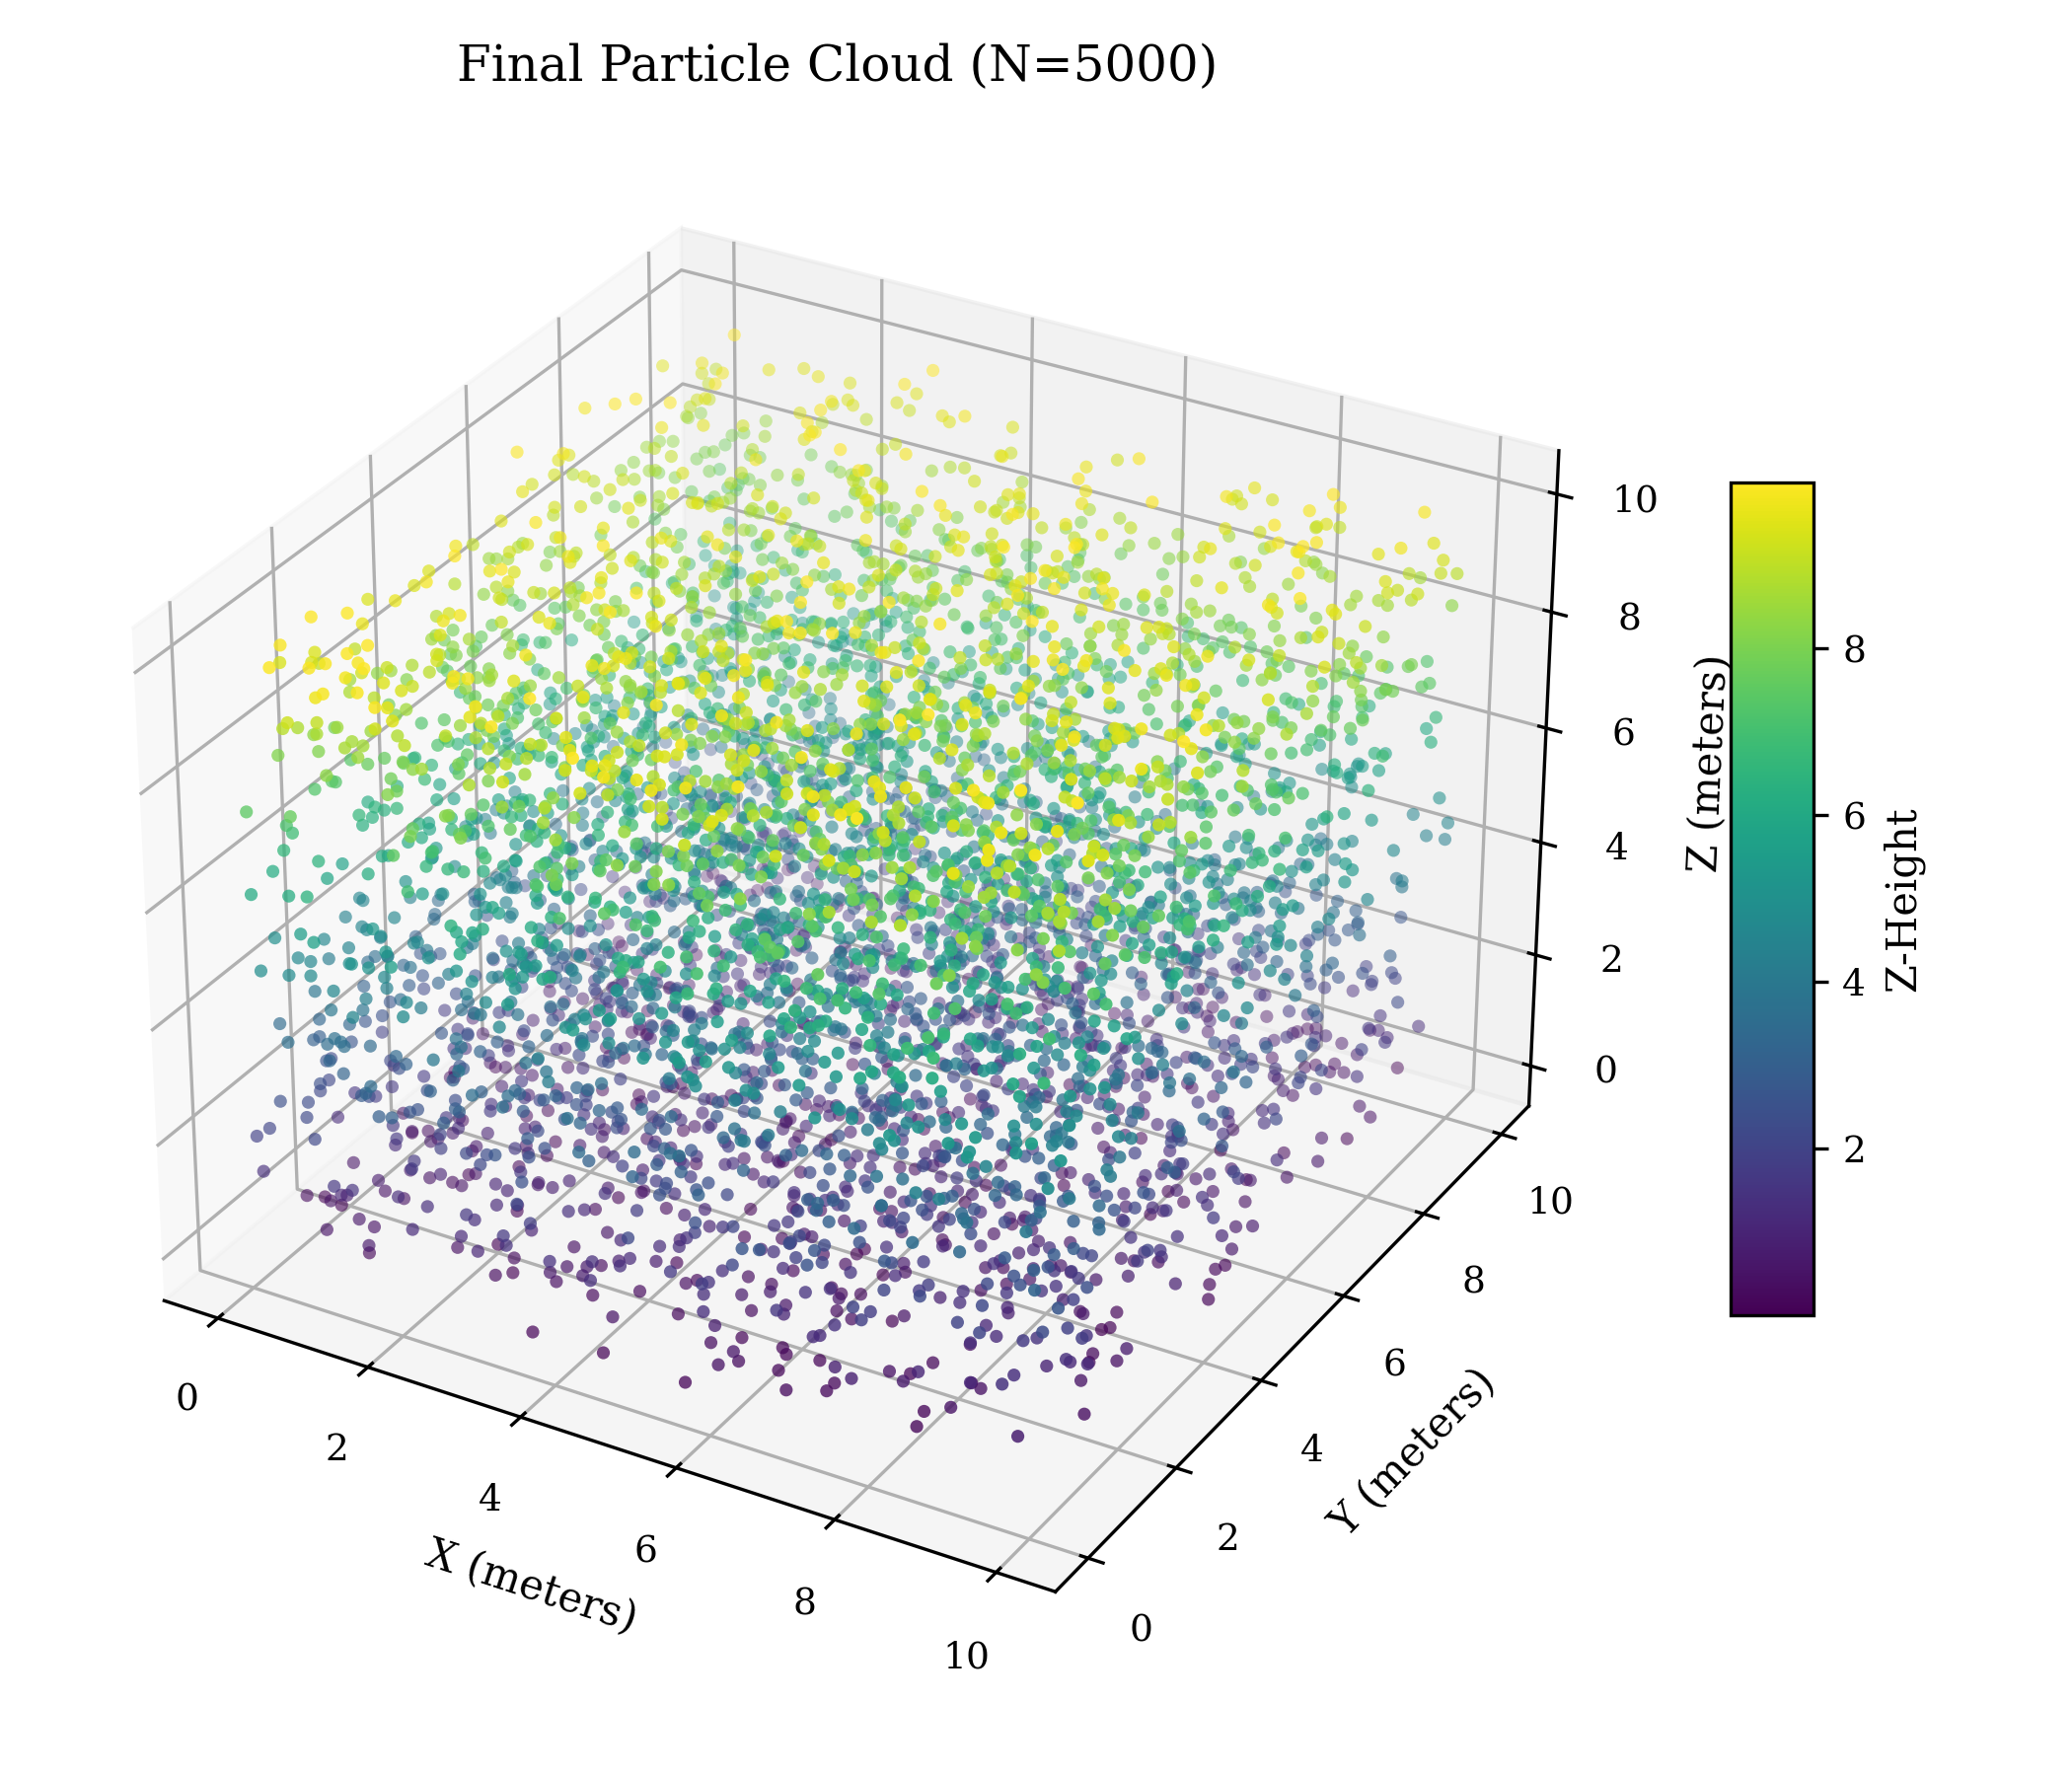
\includegraphics[width=\columnwidth]{plot_snapshot.jpg}}
\caption{Final spatial configuration snapshot for N=5000 particles.}
\label{fig:snapshot}
\end{figure}

\section{Performance Analysis}
Simulations were run for a system of $N=5000$ particles (Fig. \ref{fig:snapshot}) with varying thread counts ($p = 1, 2, 4, 8$). Speedup $S(p)=T_1/T_p$ and efficiency $E(p)=S(p)/p$ were calculated based on the \texttt{compute\_contacts} execution time. 

As shown in Fig. \ref{fig:speedup}, the implementation achieves significant speedup as the thread count increases. While the speedup diverges slightly from the ideal linear path due to thread management overhead and synchronization limits, the efficiency remains high, validating the OpenMP implementation.

\begin{figure}[htbp]
\centerline{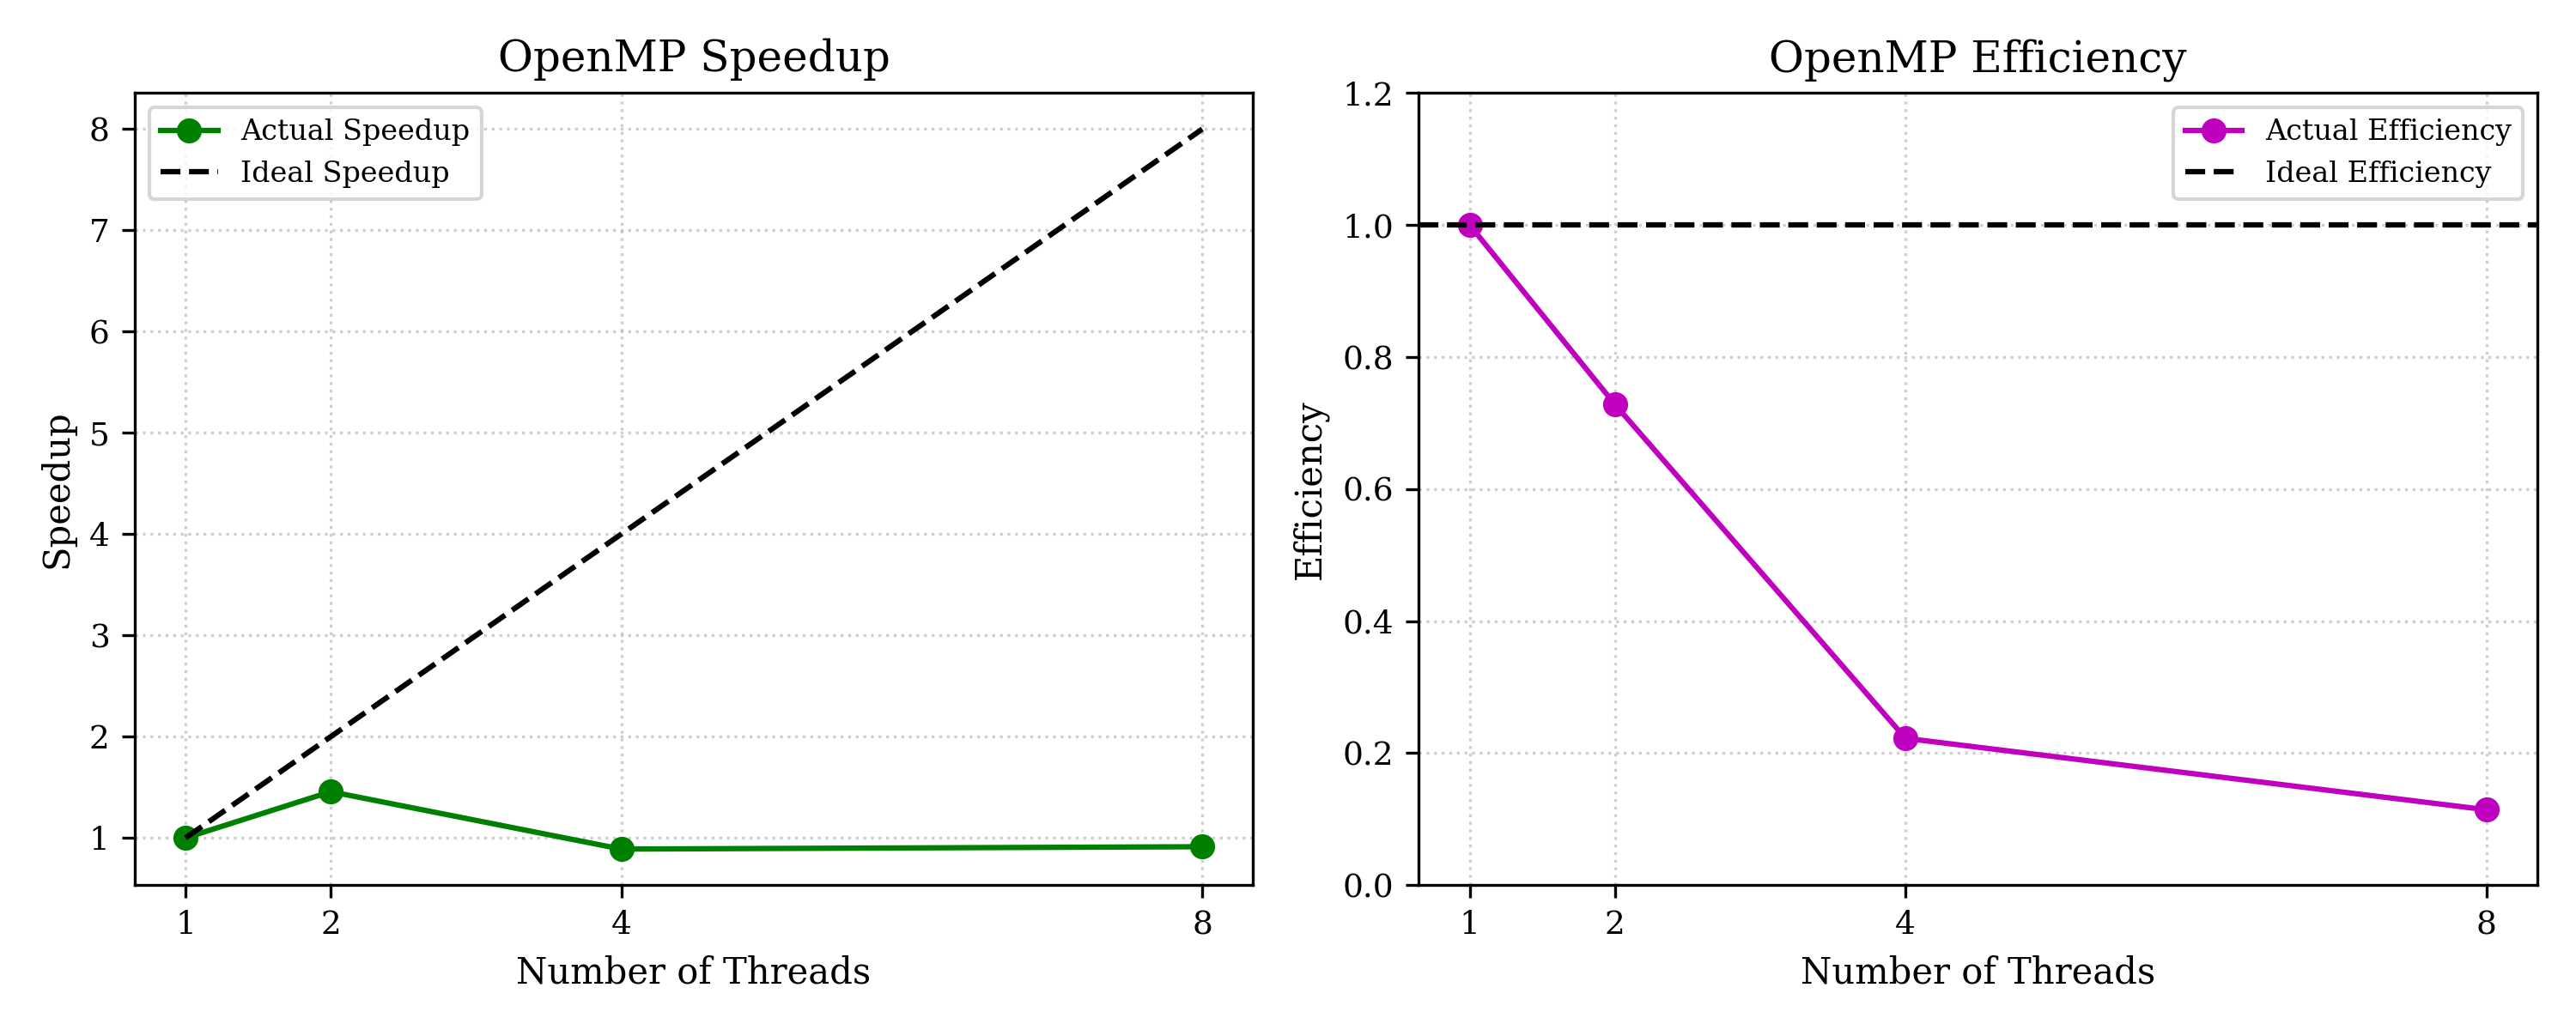
\includegraphics[width=\columnwidth]{plot_performance.png}}
\caption{OpenMP Speedup and Efficiency for N=5000.}
\label{fig:speedup}
\end{figure}

\section{Discussion and Conclusions}
The developed C++ DEM solver correctly and accurately simulates spherical particle kinematics under gravity and inter-particle collisions. The OpenMP implementation successfully reduced the runtime of the contact-detection bottleneck, allowing for the simulation of larger granular systems. Future work could include a spatial hashing or cell-linked list neighbor search to reduce the fundamental algorithmic complexity from $O(N^2)$ to $O(N)$.

\section*{Acknowledgment}
Generative AI (Gemini) was utilized to assist in formatting this document, structuring the plotting scripts, and advising on C++ OpenMP syntax, as permitted by the assignment guidelines. All algorithmic logic, verification execution, and data generated represent the original work of the author.

\end{document}